\section{Objetivos}
O presente trabalho tem por objetivo construir uma curva de EFV (do
ingês, \emph{equilibrium flash vaporization}) para um petróleo qualquer. A
composição do óleo será determinada a partir de valores de TBP (do ingês,
\emph{true boiling point} - ponto de ebulição verdadeiro) obtidos de
informações fornecidadas pelo site da TOTSA.

\section{Introdução teórica}

\subsection{TBP}
A curva de TBP (\emph{true boiling point}) ou PEV (ponto de ebulição verdadeiro)
é um gráfico que contem os valores dos pontos de ebulição  dos componentes quase puros q
ue estão contidos em um petróleo bruto ou em alguma de suas frações. Antigamente, 
essa curva era construída em laboratório utilizando equipamentos complexos de 
destilação em batelada com cem ou mais estágios de equilíbrio e alta razão de 
refluxo. Hoje em dia, esse mesmo gráfico é feito por meio de espectroscopia de massa, 
muito mais rápida e com precisão mais elevada. Uma curva típica dessa análise está 
apresentada na Figura 1 \cite{Jones2006}.

\subsection{EFV}


A curva EFV (\emph{equilibrium flash vaporization}) fornece a informação da
temperatura que um dado volume de destilado será vaporizado. Esse vapor
destilado está sempre em equilíbrio com a fase líquida e os ensaios de EFV são
sempre conduzidos em pressão atmosférica. De acordo com \citeonline{Eckert2008},
esse ensaio é raramente realizado, pois é muito trabalhoso. Em uma série de
experimentos, são medidas as temperaturas de equilíbrio para diferentes valores especificados de 
 fração de líquidos. Esse tipo de ensaio também é usado para projetar processos
 onde ocorre equilíbrio líquido-vapor como, por exemplo, refervedores, condesadores
  parciais, etc).

\subsection{Regras de Mistura}
\citeonline{Koretsky2013} afirma que a abordagem mais prática no uso de equações de estado
é utilizar regras de mistura que se baseiam nos dados dos componentes puros e 
aplicam tais para os tipos de interações presentes na mistura em questão. A 
\autoref{eq:aij} apresenta a formulação para o termo relacionado à força de
atração entre duas moléculas diferentes em uma mistura.

\begin{equation}\label{eq:aij}
a_{mix} = \sum_i\sum_jy_iy_ja_{ij}
\end{equation}
onde y são as frações molares dos componentes $i$ e $j$ e $a_{ij}$ é a
atração entre as molecúlas dos mesmos componentes $i$ e $j$. O termo de atração
da \autoref{eq:aij2} segue as premissas apresentadas a seguir:

\begin{equation}\label{eq:aij2}
a_{ij} = a_{ji}
\end{equation}

\begin{equation}\label{eq:aij3}
a_{ij} = \sqrt{a_ia_j}(1 - k_{ij})
\end{equation}

\begin{equation}\label{eq:aij4}
a_{i} = a_{ii}
\end{equation}

A \autoref{eq:bmix} apresenta a relação para o termo relacionado ao volume
excluído quando ocorre a mistura.

\begin{equation}\label{eq:bmix}
b_{mix} = \sum_iy_ib_i
\end{equation}

\subsubsection{SCMR}
\citeonline{Staudt2012} afirmam que esta regra de mistura
apresenta volume de excesso negligenciável e a fração $ u =
\frac{V}{b} $ é constante.

\subsubsection{PSRK}

\citeonline{Chen2002} afirma que o paramêtro a pode ser calculado a partir
da \autoref{eq:abrt}.


\begin{equation}\label{eq:abrt}
\frac{a}{bRT} = \sum x_i\frac{a_{ii}}{b_iRT}+\frac{1}{A}\left (
\frac{g_0^E}{RT}+\sum x_iln\frac{b}{b_i} \right )
\end{equation}
onde $A$ foi setado como -0,64663. \citeonline{Fischer1996} afirmam
que PSRK geram bons resultados para as propriedades termodinâmicas, especialmente para 
equilíbrios líquido-vapor em altas pressões.

\subsection{Modelo de Atividade: Scatchard-Hildebrand}
Segundo \citeonline {Brignole2013}, a teoria de soluções regulares de
Scatchard-Hildebrand provém do modelo de Flory-Huggins considerando que a entropia da mistura corresponde ao valor 
de uma mistura ideal. Além disso, ela leva em consideração a existência do 
calor da mistura que ocorre devido às interações energéticas moleculares. 
Uma vez que todas as combinações em uma mistura binária sejam levadas em 
conta, a expressão para o coeficiente de atividade do componente 1 é
apresentada na \autoref{eq:lngamma1}:

\begin{equation}\label{eq:lngamma1}
ln\gamma_1 = \frac{\nu_1\varphi_2^2(\delta_1-\delta_2)^2}{RT}
\end{equation}
onde $\gamma_1$é o coeficiente de atividade e $\nu_1$ é o volume molar para o
componente 1 e $\varphi_2$é a fração volumétrica do componente 2. Os parâmetros
de solubilidade dos componentes puros ($\delta_1$ e $\delta_2$ ) podem ser
obtidos a partir da energia interna de vaporização de cada componente puro $i$
($\Delta u_i^v$), como um líquido saturado na temperatura do sistema
(\autoref{eq:deltai}):

\begin{equation}\label{eq:deltai}
\delta_i = \left ( \frac{\Delta u_i^V}{\nu_i^L} \right )^{\frac{1}{2}}
\end{equation}

O termo entre parânteses é denominado de densidade de energia coesiva e o
parâmetro de solubilidade para misturas multicomponentes é mostrada a seguir:

\begin{equation}\label{eq:delta}
\delta = \sum_i\sum_j\phi_i\phi_j\delta_{ij}^2
\end{equation}

onde,

\begin{equation}\label{eq:deltaij}
\delta_{ij}^2 = \delta_1\delta_j
\end{equation}

Assim,

\begin{equation}\label{eq:delta2}
\delta = \sum_i\phi_i\delta_i
\end{equation}

\clearpage
\section{Metodologia}

\subsection{Dados experimentais}

Estão apresentados na \autoref{tab:dados}.

\begin{table}[htb]
\renewcommand{\arraystretch}{1.3}
\caption{Característica do petróleo extraída do poço CLOV - Angola}
\footnotesize 
\center
\begin{tabular}{llc}
\toprule
 {Data da análise}						&						&	{25/01/20016}	\\
 {Densidade a 15$^\circ$C (kg/m$^3$)}	&						&	{858,9}			\\
 {$^\circ$API}							&						&	{33,2}			\\
 {Bbl/mt}								&						&	{7,336}			\\
 {Acidez (mg KOH/g)}					&						&	{0,54}			\\
 {Enxofre (massa\%)}					&						&	{0,249}			\\
 {Sulfeto de Hidrogênio (mg/kg)}		&						&	{1}				\\
 {Enxofre de mercaptanos (mg/kg)}		&						&	{3}				\\
 {Viscosidade (cSt)} 					&		{10 $^\circ$C}	&	{19,3}			\\
 { }				 					&		{50 $^\circ$C}	&	{5,4}			\\
 {Ponto de Fluidez ($^\circ$C)}			&						&	{-6}			\\
 {Nitrogênio total (massa\%)}			&						&	{0,142}			\\
 {Cera (massa\%)}						&						&	{-}				\\
 {Temp. aparente de cera  ($^\circ$C)}	&						&	{-}				\\
 {RVP a 37,8 $^\circ$C (kPa)}			&						&	{26}			\\
 {Umidade (vol\%)}						&						&	{-}				\\
 {NaCl (mg/kg)}							&						&	{-}				\\
 {Níquel (mg/kg)}						&						&	{7,7}			\\
 {Vanádio (mg/kg)}						&						&	{1,9}			\\
 {Ferro (mg/kg)}						&						&	{-}				\\
 {Mercúrio ($\mu$g/kg)}					&						&	{-}				\\
 {Leves (vol\%)}						&	{Etano}				&	{0,06}			\\
 										&	{Propano}			&	{0,57}			\\
 										&	\emph{iso}-Butano	&	{0,33}			\\
 										&	\emph{n}-Butano		&	{0,94}			\\
\bottomrule
\multicolumn{3}{c}{Fonte: \citeonline{TOTSA2016}}
\end{tabular}
\label{tab:dados}
\end{table}
\clearpage

Estão apresentados na \autoref{tab:tbp}.

\begin{table}[htb]
\renewcommand{\arraystretch}{1.3}
\caption{Dados experimentais do equilíbrio líquido-vapor da mistura
etano(1)/propeno(2) a 100 ºF.}
\sisetup{table-format=2.2,round-mode=places,round-precision=2}
\footnotesize
\center
\begin{tabular}{S[table-format=3.0,round-mode=places,round-precision=0]SS|S[table-format=3.0,round-mode=places,round-precision=0]SS}
\toprule
   {T} & {\%. vap.} & {\% vap.}&{T} &
   {\% vap.} & {\% vap.}\\
   {($^\circ$C)} & {(massa)} & {(vol.)}&{($^\circ$C)} &
   {(massa)} & {(vol.)}\\
\midrule 
80  &4.88  &6.60&  340 & 49.61 &53.57\\
90  &5.83  &7.73&  360 & 53.30 &57.18\\
100 &7.01  &9.10&  380 & 56.86 &60.64\\
120 &10.02 &12.54& 400 & 60.31 &63.96\\
140 &13.62 &16.56& 420 & 63.66 &67.16\\
160 &17.05 &20.31& 440 & 66.91 &70.25\\
180 &19.98 &23.47& 460 & 70.06 &73.22\\
200 &22.86 &26.52& 480 & 73.09 &76.05\\
220 &26.08 &29.90& 500 & 75.99 &78.75\\
240 &29.72 &33.65& 520 & 78.73 &81.28\\
260 &33.64 &37.67& 540 & 81.30 &83.64\\
280 &37.71 &41.78& 560 & 83.68 &85.81\\
300 &41.78 &45.85& 580 & 85.87 &87.80\\
320 &45.76 &49.80&     &       &     \\
\bottomrule
\multicolumn{6}{c}{Fonte: \citeonline{TOTSA2016}}
\end{tabular}
\label{tab:tbp}
\end{table}
\clearpage 

\clearpage
\section{Resultados} 


\begin{table}[htb]
\renewcommand{\arraystretch}{1.3}
\caption{Dados experimentais do equilíbrio líquido-vapor da mistura
etano(1)/propeno(2) a 100 ºF.}
\sisetup{table-format=2.2,round-mode=places,round-precision=2}
\footnotesize
\center 
\begin{tabular}{lccc}   
\toprule
   &{Temperatura Inicial}&{Temperatura Final}&\multirow{2}{*}{$\Delta$T} \\
  &{da Fração Vaporizada ($^\circ$C)}&{da Fração Vaporizada
   ($^\circ$C)} & \\
\midrule 
{EFV: PR+SCMR}	&	73	&	472		&	1 \\
{EFV: PR+VDW}	&	75	&	468		&	1 \\
{EFV: PR+PSRK}	&	51	&	469		&	1 \\
\bottomrule
%\multicolumn{4}{c}{Fonte: \citeonline{TOTSA2016}}
\end{tabular}
\label{tab:result1}
\end{table}
\clearpage 

\begin{table}[htb]
\renewcommand{\arraystretch}{1.3}
\caption{blablabla}
\sisetup{table-format=2.2,round-mode=places,round-precision=2}
\footnotesize
\center 
\begin{tabular}{lcc}   
\toprule
  {Regras de Mist.} &{Máx. Diferença}&{Faixa de Máx.} \\
   {Comparadas}&{do \% Vaporizada}&{diferença de T ($^\circ$C)} \\
\midrule 
{SCMR - vdW}	&	1.34	&	{256 - 257}	 \\
{SCMR - PSRK}	&	2.55	&	{151 - 159}	 \\
{vdW - PSRK}	&	1.88	&	{112 - 118}	 \\
\bottomrule
%\multicolumn{4}{c}{Fonte: \citeonline{TOTSA2016}}
\end{tabular}
\label{tab:result2}
\end{table}
\clearpage



Conforme ilustra a \autoref{fig:efv}.

\begin{figure}[htb]
\centering
{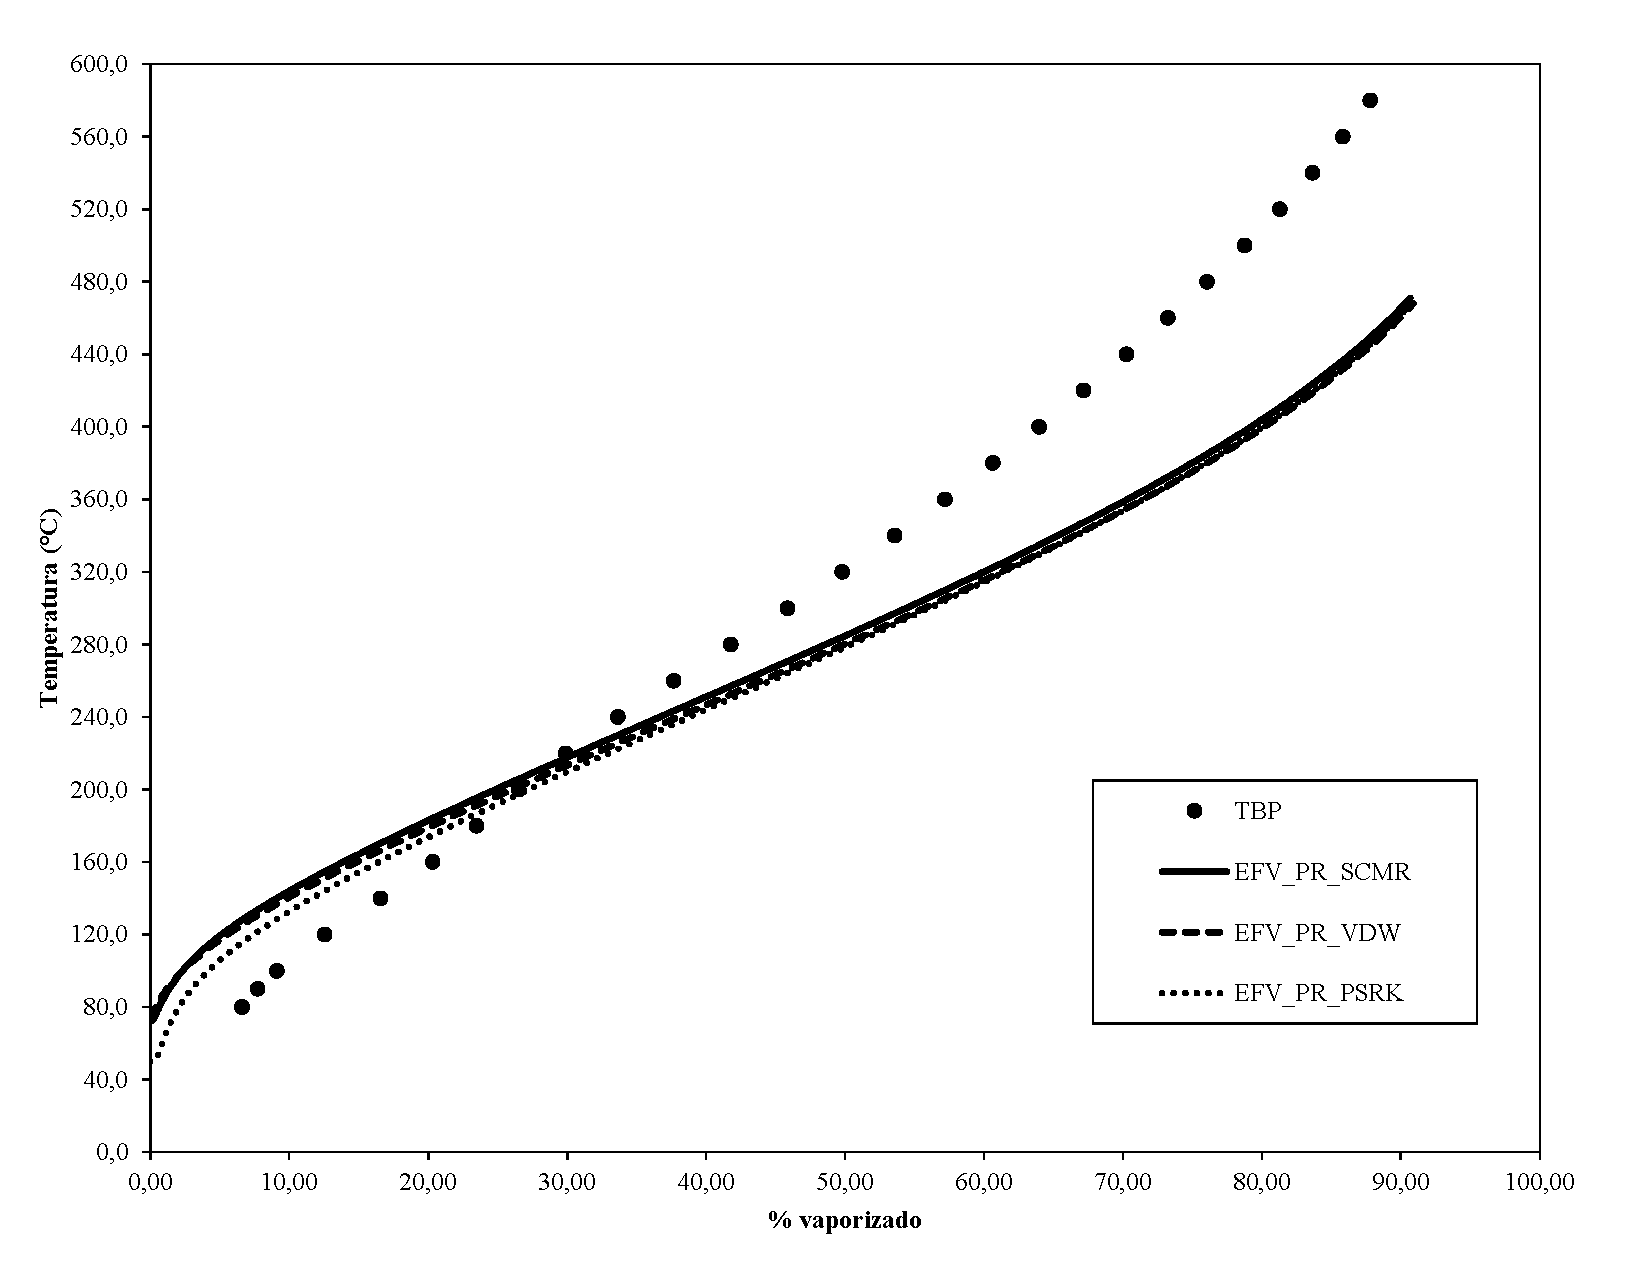
\includegraphics[width=1.0\textwidth]{img/trab3.pdf}} 
\caption{Curva de TBP e EFV para o petróleo do poço CLOV - Angola}
\label{fig:efv}
\end{figure} 

\begin{figure}[htb]
\centering
{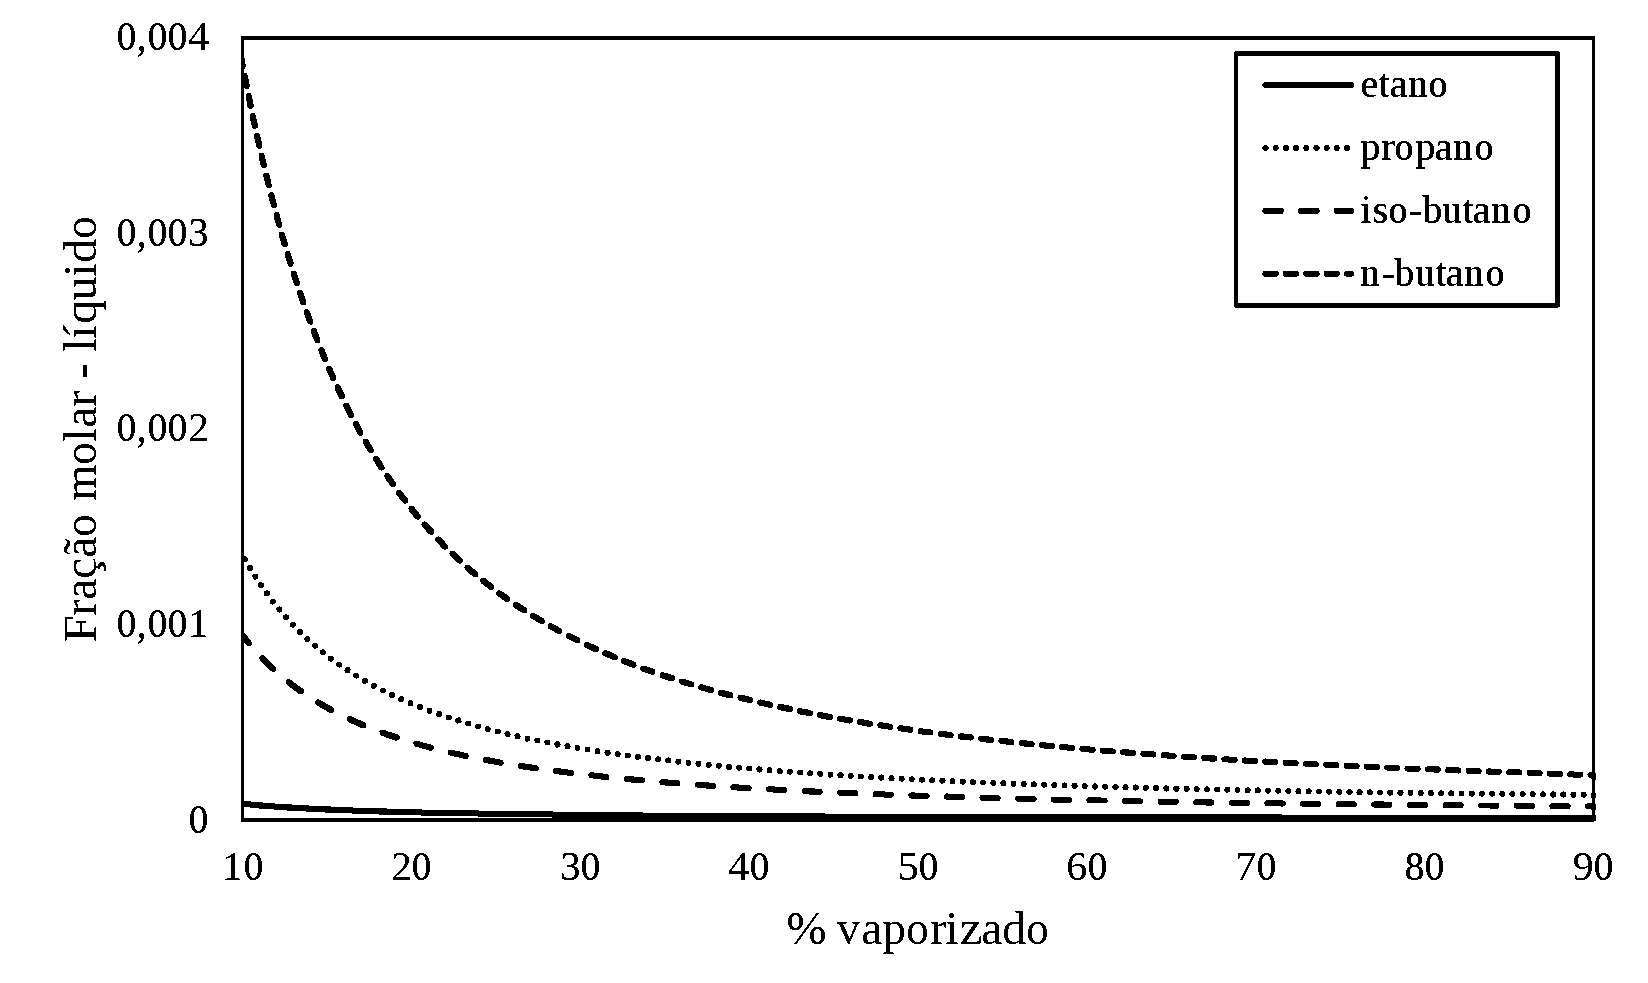
\includegraphics[width=1.0\textwidth]{img/trab3liq.pdf}} 
\caption{Composição dos leves no produto de fundo em função do
percentual vaporizado}
\label{fig:liq}
\end{figure}

\begin{figure}[htb]
\centering
{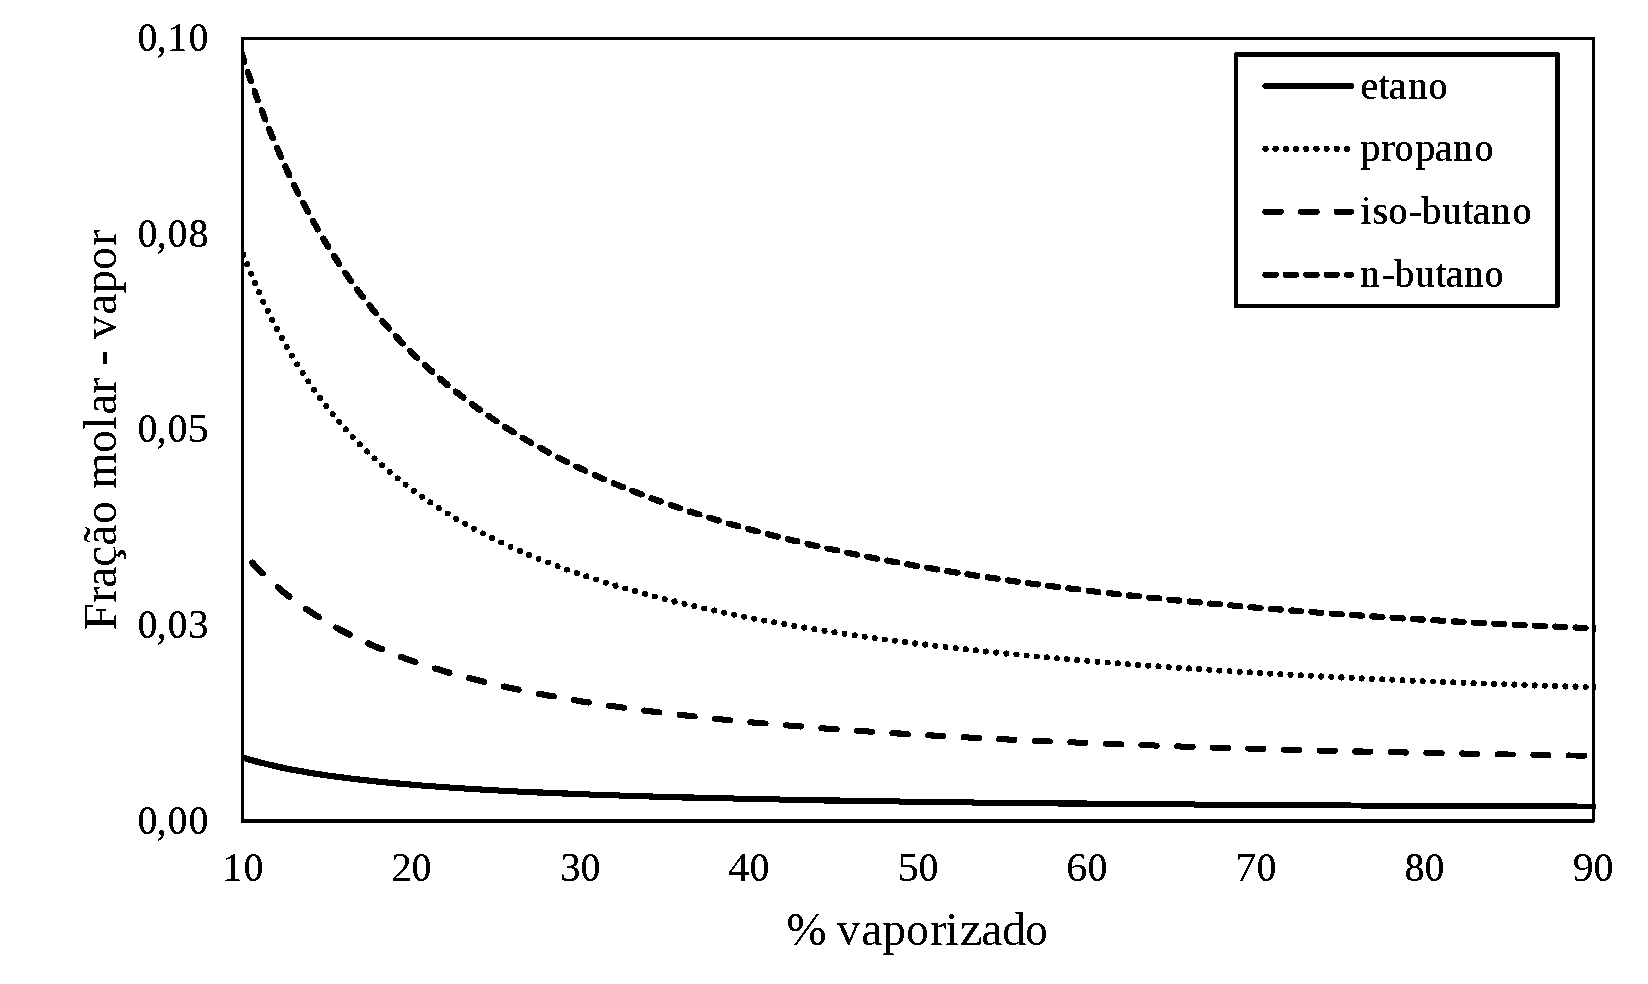
\includegraphics[width=1.0\textwidth]{img/trab3vap.pdf}} 
\caption{Composição dos leves no produto de topo em função do percentual
vaporizado}
\label{fig:vap}
\end{figure}

\begin{figure}[htb] 
\centering
{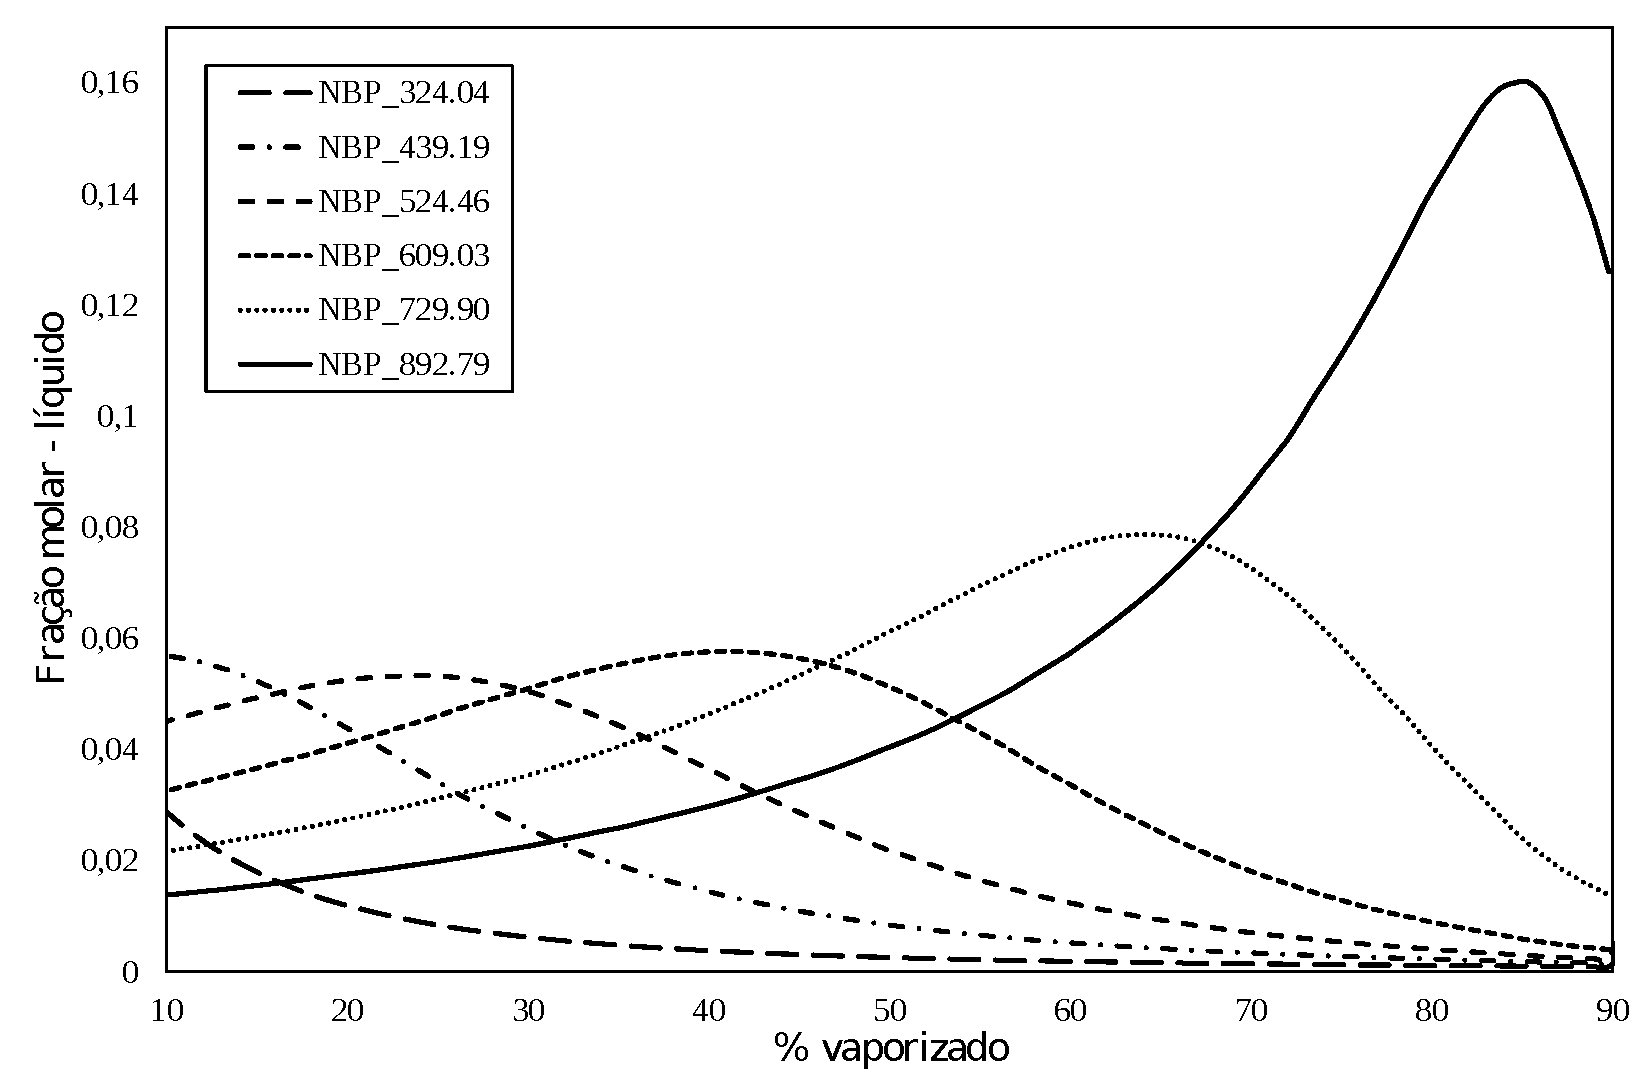
\includegraphics[width=1.0\textwidth]{img/trab3liqall.pdf}} 
\caption{Composição de alguns pseudos no produto de fundo em função do
percentual vaporizado}
\label{fig:liqall}
\end{figure}

\begin{figure}[htb]
\centering
{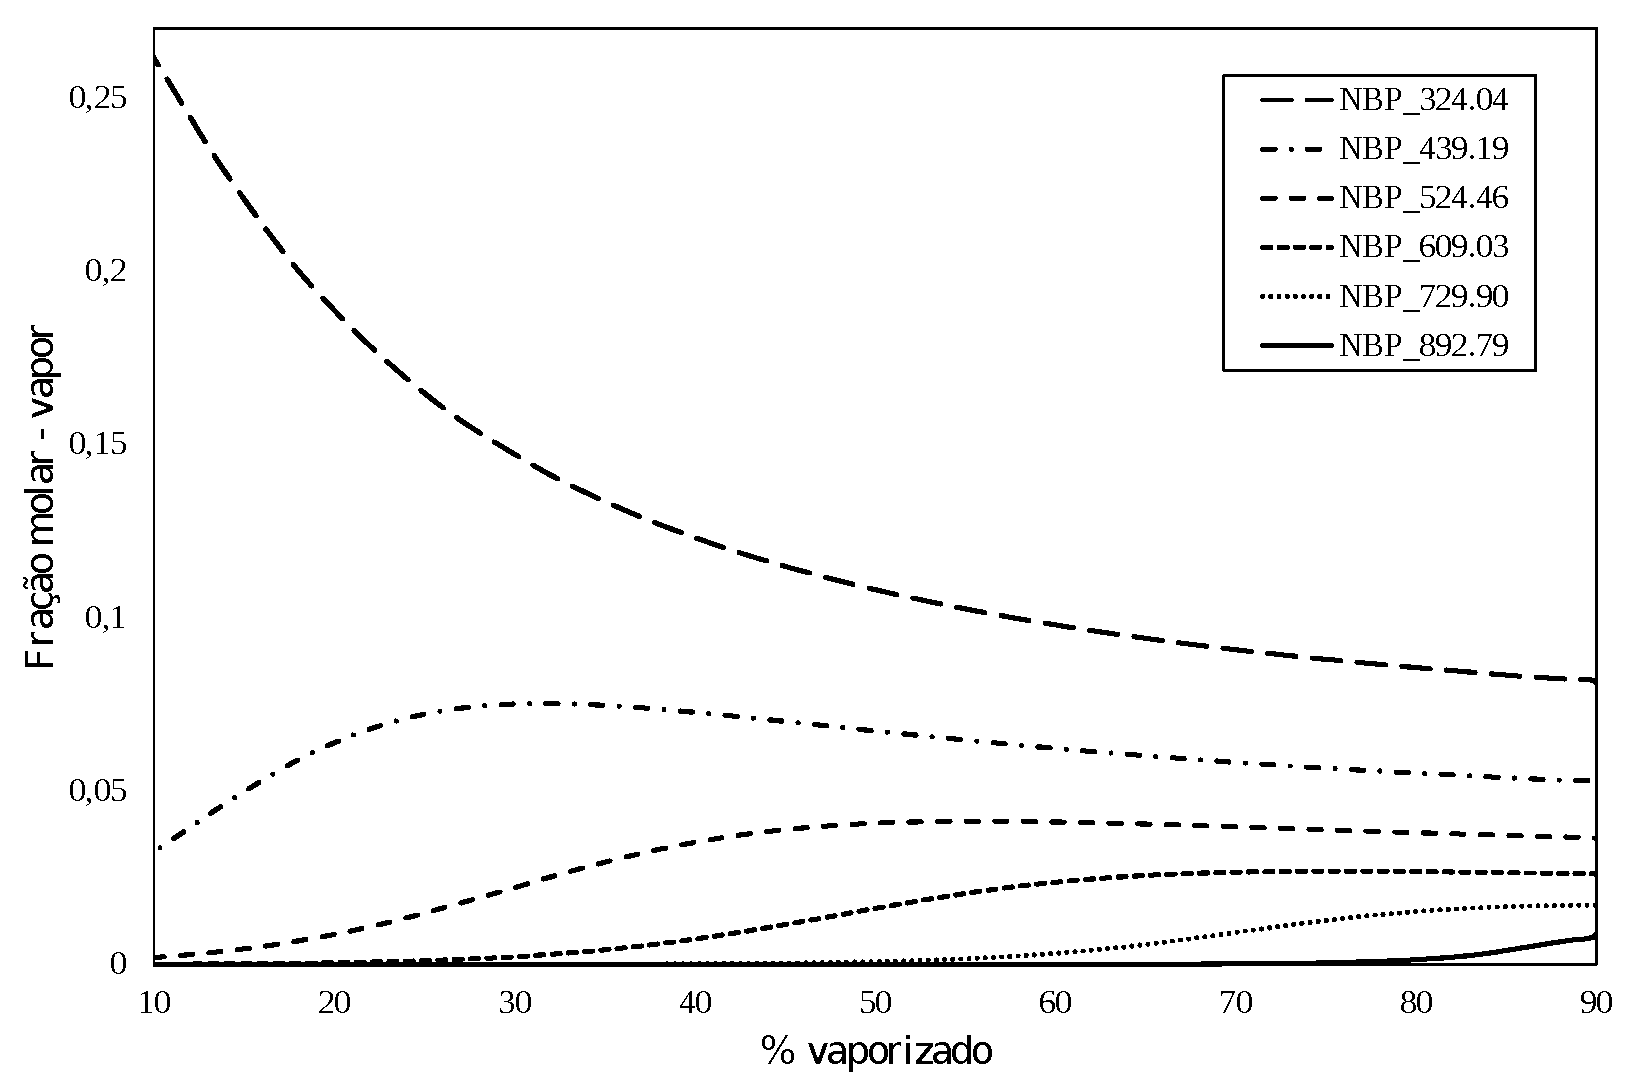
\includegraphics[width=1.0\textwidth]{img/trab3vapall.pdf}} 
\caption{Composição de alguns pseudos no produto de topo em função do
percentual vaporizado}
\label{fig:vapall}
\end{figure}

\clearpage
\section{Conclusões} 

